\section{LLM-Based Agent Frameworks}
\label{sec:agent-frameworks}

The development of LLM-based agents has accelerated rapidly, with numerous frameworks emerging to facilitate the creation of AI systems that can reason, plan, and take actions~\cite{cheng2024llmagents}. This section surveys relevant agent frameworks and patterns that inform the design of the Slurm Agent system.

\subsection{Agent Paradigms}

LLM-based agents extend language models beyond text generation to systems capable of interacting with external environments. Several paradigms have emerged:

\textbf{ReAct (Reason + Act)} combines reasoning and acting in an interleaved manner. The agent alternates between generating reasoning traces (thoughts) and taking actions, using observations from actions to inform subsequent reasoning. This pattern enables transparent decision-making and effective problem decomposition.

\textbf{Chain-of-Thought (CoT)} prompting encourages models to generate intermediate reasoning steps before producing final answers. When combined with tool use, CoT enables agents to plan multi-step solutions and verify their progress.

\textbf{Reflexion} introduces self-reflection mechanisms where agents evaluate their own outputs and learn from mistakes within a single episode. Failed attempts generate feedback that informs subsequent tries, improving performance without parameter updates.

\textbf{Tree-of-Thoughts (ToT)} extends linear reasoning to explore multiple reasoning paths simultaneously. The agent evaluates alternative approaches and can backtrack when one path proves unproductive.

\subsection{Framework Implementations}

Several open-source frameworks provide infrastructure for building LLM-based agents:

% Placeholder: Agent framework comparison diagram
\begin{figure}[H]
    \centering
    % \fbox{\parbox{0.8\textwidth}{\centering \textit{[Placeholder: Comparison diagram of different agent frameworks and their architectures]}}}
    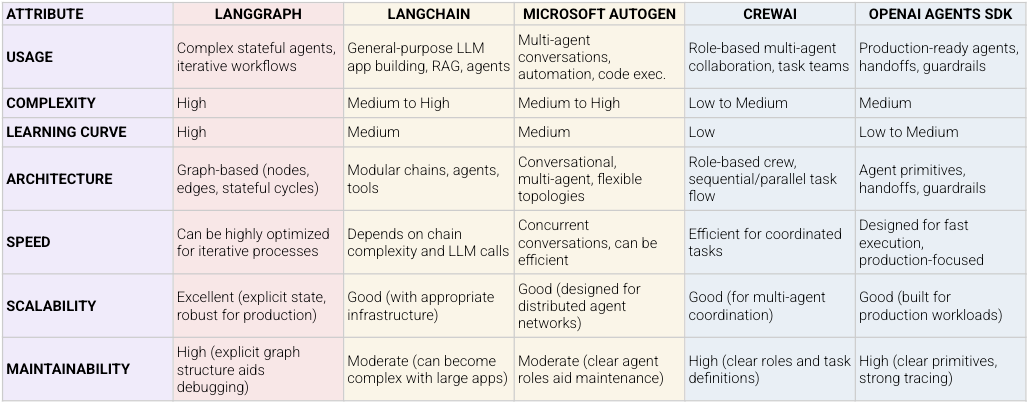
\includegraphics[width=1\textwidth]{images/agent_frameworks_comparison.png}
    \caption{Comparison of LLM Agent Frameworks}
    \label{fig:agent-frameworks}
\end{figure}

\subsection{Multi-Agent Systems}

Complex tasks often benefit from multiple specialized agents working together. Multi-agent architectures divide responsibilities among agents with distinct capabilities:

\textbf{Hierarchical architectures} employ a coordinator agent that delegates subtasks to specialized worker agents. The coordinator maintains overall task state and synthesizes results from workers.

\textbf{Collaborative architectures} enable peer agents to communicate and coordinate without central control. Agents may negotiate, share information, or critique each other's outputs.

\textbf{Handoff patterns} allow one agent to transfer control to another when the task requires different capabilities. The receiving agent continues execution with relevant context from the handoff.

The OpenAI Agents SDK specifically supports handoff patterns, where agents can transfer conversations to other agents based on task requirements. This mechanism enables modular agent design where each agent focuses on specific capabilities.

\subsection{Tool Integration Patterns}

Effective agent systems require robust tool integration. Common patterns include:

\textbf{Direct function calling}: Tools are defined as functions that the LLM can invoke directly. This approach is simple but couples tool definitions to the agent implementation.

\textbf{Plugin architectures}: Tools are packaged as plugins that can be dynamically loaded and configured. This enables extensibility without modifying core agent code.

\textbf{Protocol-based integration}: Tools are exposed through standardized protocols (such as MCP), enabling interoperability across different agent frameworks and tool providers.

The protocol-based approach offers significant advantages for maintainability and reusability. Tools developed for one agent system can be used with others, and tool implementations can evolve independently of agent logic.

\subsection{Relevance to Slurm Agent}

The Slurm Agent design draws on lessons from existing frameworks:
\begin{itemize}
    \item The ReAct pattern informs the agent's approach to reasoning about Slurm operations
    \item Multi-agent architecture with handoffs enables specialized handling of different task types
    \item The OpenAI Agents SDK provides the implementation foundation
    \item MCP-based tool integration ensures modularity and security
\end{itemize}

By combining proven patterns with domain-specific design, the Slurm Agent addresses the unique requirements of HPC cluster management while leveraging established best practices from the agent development community.

\subsection{Domain-Adapted Fine-Tuning for Tool-Use Agents}

A growing body of work explores fine-tuning open-weight models specifically for tool-calling and agentic behavior, aiming to replicate commercial API capabilities at lower cost and with local deployment.

\textbf{ToolLLM}~\cite{qin2023toolllm} constructs a dataset of 16{,}000+ tool-use trajectories by prompting a teacher model (ChatGPT) to solve tasks requiring API calls from a large tool repository. A smaller model (LLaMA) is then fine-tuned on these trajectories, achieving tool-selection accuracy competitive with the teacher on the held-out ToolBench benchmark. The key insight is that high-quality tool-use data can be synthesized from evaluation rather than manually annotated.

\textbf{Gorilla}~\cite{patil2023gorilla} fine-tunes LLaMA-7B on API documentation and usage examples, demonstrating that domain-specific fine-tuning dramatically reduces API hallucination---generating calls to non-existent functions or using incorrect argument formats. Gorilla shows that smaller models with focused training can outperform GPT-4 on structured API generation tasks within their training domain.

\textbf{AgentTuning}~\cite{zeng2023agenttuning} demonstrates that fine-tuning on a mix of agent interaction trajectories across multiple environments generalizes well to unseen agent tasks. The work shows that trajectory-based training---where the model learns complete episodes of reasoning, action, and observation---is more effective than training on isolated instruction-response pairs.

These approaches share common principles with this thesis: (1)~using evaluation-validated traces as training signal rather than manual annotation, (2)~focusing fine-tuning on the tool-calling and decision-making layers rather than general language capability, and (3)~demonstrating that smaller domain-adapted models can approach larger general-purpose models within their operational scope. The Slurm Agent's fine-tuning contribution extends this line of work by introducing role-scoped tool exposure---enforcing the Observer/Operator safety boundary directly in the training data format---which is novel relative to prior flat-tool-list approaches.
